\documentclass[letterpaper,twocolumn,10pt]{article}
\usepackage{usenix2020}

% to be able to draw some self-contained figs
\usepackage{tikz}
\usepackage{amsmath}
\microtypecontext{spacing=nonfrench}

%-------------------------------------------------------------------------------
\begin{document}
%-------------------------------------------------------------------------------

%don't want date printed
\date{}

% make title bold and 14 pt font (Latex default is non-bold, 16 pt)
\title{\Large \bf MPKLink: Performant \& Trusted Microservice Communication with Intel Memory Protection Keys}

\author{
{\rm Salma Alandary}\\
\url{ssalandary@ucla.edu}\\
University of California, Los Angeles (UCLA)
\and
{\rm Benson Liu}\\
\url{bensonhliu@ucla.edu}\\
University of California, Los Angeles (UCLA)
} % end author

\maketitle

%-------------------------------------------------------------------------------
\begin{abstract}
When multiple microservices are co-located on the same machine, one common optimization is to take advantage of shared memory for communication.
Shared memory allows different processes to access a common memory region, leading to faster data transfer compared to traditional network-based methods.
However, shared memory primitives introduce several challenges, including a lack of fine-grained access control, synchronization overhead, and copying overhead.
Fine-grained access control is necessary to ensure that only authorized processes can read from or write to specific memory regions, while synchronization overhead arises when processes must coordinate access to prevent race conditions.
Additionally, many shared memory systems require copying data between different buffers, further increasing the overhead.
Intel Memory Protection Keys (MPK) provide a hardware-backed solution to these problems by enabling processes to control access to memory pages with fine-grained protection keys, thus reducing the need for complex synchronization mechanisms and eliminating unnecessary data copying.
In response to these challenges, we propose MPKLink, a system that enables performant and trustworthy communication between microservices hosted on the same machine.
MPKLink provides a framework for making small modifications to microservice orchestration software like Docker Compose and a gRPC compiler, allowing microservices to communicate securely via Intel MPK with minimal changes to their existing codebase.
To assess its effectiveness, we benchmarked various inter-process communication (IPC) primitives, including OS pipes, Unix domain sockets, shared memory, and Intel MPK, comparing their performance and highlighting the advantages of using Intel MPK for high-performance, secure inter-service communication.
After evaluating MPKLink against communication methods such as OS pipes, Unix domain sockets, and shared memory, we concluded that while it performs comparably to or better than at least one of these IPC methods for smaller-scale communications, it faces challenges with larger reads and writes. Although MPKLink is consistently slower than a bare shared memory implementation, it offers stronger isolation guarantees, making it more suitable for threat models requiring higher security. We believe that the efficiency of MPKLink can be further improved by optimizing shared memory spinlocks to use atomic variables, allowing each thread to modify its Protection Key Rights for User pages (PKRU) register at appropriate times. Additionally, identifying and eliminating unnecessary memory copying could reduce overhead. While these enhancements may not enable MPKLink to outperform Unix domain sockets or OS pipes for large data transfers, they present promising research directions for applications with smaller-scale or high-frequency inter-service communication. By addressing these limitations, MPKLink has the potential to become a more versatile and efficient solution for secure microservice communication.
\end{abstract}


%-------------------------------------------------------------------------------
\section{Introduction}
Microservices have revolutionized the way modern applications are developed, enabling modularity, scalability, and maintainability by breaking down monolithic systems into discrete, loosely coupled services.
However, as microservices proliferate, especially when hosted on the same machine, the traditional methods of inter-microservice communication—such as Remote Procedure Calls (RPCs) or REST APIs—can become bottlenecks.
These approaches rely on network-like communication stacks that introduce unnecessary overhead when services share the same physical host.
One potential optimization when microservices are co-located on the same machine is to leverage shared memory for communication.
This approach can significantly reduce latency and improve throughput by bypassing the network stack and directly accessing memory.

Recent trends in research and industry highlight the inefficiencies in conventional inter-microservice communication paradigms.
Most existing systems still rely on REST, gRPC, or Thrift for communication, secured via methods such as JSON Web Tokens (JWT) or mutual TLS.
While these approaches are effective for distributed services, they are suboptimal for co-located microservices that could directly share memory.
The inefficiency arises from the multiple layers of abstraction and the reliance on protocols designed for remote communication, which are unnecessary for services sharing the same host.
Thus, there is a growing need to explore alternatives that balance performance with critical aspects like isolation and security.

\subsection{Threat Model}
The threat model for MPKLink assumes a scenario where multiple microservices are running on the same host machine.
This setup is common in modern containerized environments, such as those managed by tools like Docker Compose, where microservices operate in isolated containers but share the underlying hardware and kernel.
To enable efficient communication, these microservices often use shared memory or other inter-process communication (IPC) mechanisms facilitated by a shared filesystem mount on the host.
While this setup provides performance benefits, it introduces potential security vulnerabilities when one or more microservices become compromised.

In this threat model, the adversary is assumed to have compromised one or more microservices but not all.
They may also have gained unprivileged access to the host machine, such as through a non-root user or a service account.
With this level of access, the adversary aims to exploit shared resources like memory or the filesystem to violate the confidentiality or integrity of communication between microservices.
One key attack vector is a man-in-the-middle (MITM) attack, where the adversary intercepts or manipulates data exchanged through shared memory regions.
For instance, they might read sensitive data from the memory, tamper with it before the intended recipient reads it, or inject malicious content to disrupt the system's operation.

While containerization provides some isolation, the shared use of host resources can create pathways for adversaries to exploit.
MPKLink must address these challenges by ensuring robust protection of communication channels, safeguarding against unauthorized access, and maintaining data integrity without sacrificing the performance benefits of shared memory-based communication.

\subsection{Contributions}
In this paper, we introduce \textbf{MPKLink}, a novel system designed to enhance inter-microservice communication for co-located microservices using \textbf{Intel Memory Protection Keys (MPK)}.
While previous research involving MPK has primarily focused on using memory protection keys to safeguard memory at rest—ensuring integrity and isolation for static or infrequently accessed memory regions—MPKLink extends this concept to memory \textbf{in transit}.
By enabling dynamic and efficient communication between microservices through shared memory regions protected by MPK, our approach addresses both the performance and security challenges of traditional inter-process communication mechanisms.


MPKLink provides a practical framework for leveraging MPK to enable high-performance and trusted communication without requiring modifications to existing microservices.
By securely sharing memory protection keys between services, MPKLink facilitates communication while preserving confidentiality and integrity against adversarial threats, such as those outlined in our threat model.
We benchmark MPKLink against traditional communication protocols to demonstrate its performance benefits, analyze its isolation guarantees, and validate its compatibility with real-world microservices architectures.
Through this work, we contribute not only a novel application of MPK to inter-service communication but also a practical and deployable framework for securely accelerating microservices communication in modern containerized environments.

\section{Background}

\subsection{gRPC}
gRPC is a high-performance, open-source framework that facilitates communication between services, especially in microservice architectures.
When, for example, a Ruby service makes a gRPC call to an Android-Java service, it invokes client code generated at build time by gRPC tooling, known as a client stub.
The client stub handles encoding the data passed to it into Protocol Buffers, a language-neutral, platform-neutral binary format, which is then sent over the network to the target service.
The data is transmitted as a stream of HTTP/2 data frames, which provides multiplexing, flow control, and improved performance compared to older HTTP protocols.
Due to the binary encoding and network optimizations, gRPC is often significantly faster—up to five times faster—than using JSON over HTTP, especially for high-throughput systems.

On the receiving side, the payment service decodes the packets it receives from the network, which are in Protocol Buffers format, and invokes the corresponding server application.
The server processes the request and returns a result, which is then encoded back into Protocol Buffers format.
This result is sent through the transport layer and back to the client.
The use of Protocol Buffers for encoding ensures that data transmission is both compact and efficient, reducing the overhead associated with other data serialization methods like JSON.
Through this streamlined process, gRPC enables quick, reliable communication between microservices, making it an ideal choice for applications that require high-speed, low-latency communication.

\subsection{Inter Process Communication (IPC)}
Typically, when microservice communication falls on the same machine, this typically falls back to using different forms of inter-process communication.
\textbf{Inter-process communication (IPC)} refers to mechanisms that allow processes running on the same operating system to exchange data and coordinate their activities.
These mechanisms are essential for enabling cooperation between processes, facilitating tasks like data sharing, synchronization, and signaling.
UNIX systems provide several forms of IPC including \textbf{named pipes}, \textbf{UNIX domain sockets}, and \textbf{shared memory}.

\subsubsection{Named Pipes}
Named pipes, or FIFOs (First In, First Out), are a mechanism for inter-process communication (IPC) that allow data to flow unidirectionally between processes.
Unlike traditional pipes, which are anonymous and limited to parent-child process relationships, named pipes are represented as special files in the filesystem.
This makes them accessible to unrelated processes, facilitating communication between independently running programs.
A named pipe can be created using the \textit{mkfifo} library function which generates a pipe in the filesystem.
Processes can then interact with the named pipe using standard file operations like \textit{open}, \textit{read}, and \textit{write}, with one process writing data to the pipe and another reading from it.

A key nuance of named pipes is their inherently unidirectional nature—data flows in a single direction per pipe.
This limitation means that for bidirectional communication between two microservices, two separate named pipes must typically be created: one for sending data and the other for receiving.
This setup adds complexity, as both processes must manage the correct use of each pipe and handle potential synchronization challenges.
Additionally, since named pipes are blocking by default, a reader or writer may hang if the corresponding process is not actively interacting with the pipe, requiring careful coordination to avoid deadlocks or delays.

\subsubsection{UNIX Domain Sockets}
Unix domain sockets (UDS) are an inter-process communication (IPC) mechanism that allows efficient data exchange between processes on the same machine.
Unlike network sockets, which use protocols like TCP/IP, Unix domain sockets operate within the kernel using the \textbf{AF\_UNIX} address family.
This makes them faster and more lightweight than network communication methods.
UDS supports both stream-oriented communication, similar to TCP, and datagram-oriented communication, akin to UDP, providing flexibility for different use cases.
Because UDS exists solely on the local machine, they also offer enhanced security and reliability compared to network-based communication.

To implement communication using Unix domain sockets, the socket API can be used with the \textbf{AF\_UNIX} address family.
The process involves creating a socket file, typically with \textbf{socket(AF\_UNIX, SOCK\_STREAM, 0)} for stream-oriented communication.
One process binds the socket to a file in the filesystem using \textbf{bind()} and listens for connections with \textbf{listen()}.
Another process connects to this socket using \textbf{connect()}.
Once the connection is established, the two processes can exchange data bidirectionally using standard socket functions like \textbf{send()} and \textbf{recv()}.
For example, the server might create a socket file at \textbf{/tmp/mysocket}, and the client would use the same path to establish a connection.

A major advantage of Unix domain sockets over named pipes is their support for bidirectional communication, eliminating the need for multiple pipes to facilitate two-way data flow.
However, UDS does have some nuances.
The socket file in the filesystem must be properly managed, including cleanup after use to prevent stale files.
Additionally, because UDS operates within the kernel, it can be subject to kernel-imposed limitations such as buffer sizes, which may need tuning for performance-critical applications.
While UDS is highly efficient for local communication, it is limited to processes on the same host and cannot extend to networked systems, making it unsuitable for distributed architectures.

\subsubsection{Shared Memory}
Shared memory is a high-performance inter-process communication (IPC) method that allows multiple processes on the same system to access a common memory region directly.
This approach eliminates the overhead of copying data between processes, making it one of the fastest IPC mechanisms available.
Shared memory is particularly suitable for applications where large volumes of data need to be exchanged frequently.
However, because multiple processes access the same memory, ensuring data consistency and preventing race conditions requires additional synchronization mechanisms.

Shared memory can be implemented using the System V \textbf{shmget} API or memory-mapped files (\textbf{mmap}).
With \textbf{shmget}, a shared memory segment is created using a unique key, and processes attach to it using \textbf{shmat}.
Data can then be written to and read from the shared segment directly.
Alternatively, shared memory can be created using \textbf{mmap} by mapping a file (or using \textbf{MAP\_ANONYMOUS} for unnamed memory) into the address space of multiple processes.
Processes can access this mapped memory region as if it were a regular array.
For example, with \textbf{mmap}, processes can create a shared region backed by a file in \textbf{/dev/shm}, enabling fast communication without the need for intermediate data transfer.

One nuance of shared memory is its non-blocking nature.
Unlike pipes or sockets, shared memory does not inherently manage synchronization, meaning processes must implement their own mechanisms to avoid race conditions.
This can be done using locks, such as mutexes or semaphores, to coordinate access to the shared region.
Alternatively, separate shared memory regions can be used for reading and writing to reduce contention but at the cost of increased complexity.
Another consideration is resource management—shared memory segments must be explicitly cleaned up after use to avoid leaks, and improper handling can lead to dangling memory regions or stale data.
Despite these challenges, shared memory remains a powerful tool for achieving high-speed communication between processes on the same host.

\subsection{Problems with Shared Memory}
Using shared memory for inter-process communication (IPC) comes with several challenges, which can impact both the security and performance of applications.
These issues arise primarily because shared memory lacks built-in mechanisms for access control and synchronization, requiring developers to implement these functionalities manually.
While shared memory offers high-speed communication due to its direct memory access model, these challenges make its implementation complex and error-prone, especially in systems requiring strong security and reliability guarantees.
The key problems include:

\subsubsection{Lack of Fine-Grained Access Control}
Shared memory typically operates with broad access permissions, meaning any process that knows the shared memory key can read from or write to the region.
Since keys can often be enumerated or guessed, this creates significant risks to both confidentiality and integrity.
Unauthorized processes could access sensitive data, inject malicious content, or corrupt the memory, leading to potential security vulnerabilities.
Without additional safeguards, such as enforced policies or key obfuscation, shared memory is inherently insecure.

\subsubsection{Synchronization Overhead} 
Unlike other IPC mechanisms that inherently manage coordination, shared memory requires explicit synchronization to avoid race conditions when multiple processes attempt to read or write simultaneously.
This is typically achieved using semaphores, mutexes, or spinlocks.
However, these synchronization mechanisms introduce overhead, as processes must acquire and release locks before accessing the shared region.
Improperly managed synchronization can also lead to issues such as deadlocks, priority inversion, or performance bottlenecks in high-concurrency scenarios.

\subsubsection{Copying Overhead}
To mitigate synchronization challenges, some systems use multiple shared memory buffers, assigning specific buffers for reading and others for writing.
This approach minimizes contention, as processes access different buffers independently.
However, it doubles the copying overhead, as data must be replicated across multiple regions to maintain consistency.
This trade-off can negate some of the performance benefits of shared memory, particularly in systems where memory bandwidth is a critical resource.

\subsection{Intel Memory Protection Keys (MPK)}
Intel Memory Protection Keys (MPK) is a userspace mechanism designed to manage memory permissions more efficiently than traditional protection mechanisms.
MPK enables fine-grained control over memory access by tagging memory pages with protection keys, each associated with specific access rights such as read, write, or execute.
These protection keys are stored in the \textbf{PKRU} register, which is thread-local, meaning each thread has its own copy of the register that controls how memory pages are accessed.
The PKRU register is used at the intra-process level, allowing different threads within the same process to have distinct memory access rights for different regions of memory.
This makes MPK particularly useful for applications that require rapid, dynamic changes in memory permissions without the overhead of system calls.

One of the key advantages of MPK is its ability to manage memory permissions without the need for costly system calls like \textbf{mprotect}.
Once memory pages are tagged with protection keys, modifying the access rights to these pages can be done by simply updating the PKRU register, a much cheaper operation compared to invoking \textbf{mprotect}.
However, since the PKRU register is thread-local, its value needs to be synchronized between threads or processes to maintain consistency in memory access rights.
This synchronization can be achieved efficiently by storing the value of the PKRU register in a small shared memory region, which can be mapped between threads or processes.
This setup ensures that all participating threads or processes observe the same memory protection settings, reducing synchronization overhead while providing a flexible and fast mechanism for managing memory permissions.

\section{System Design}
Intel MPKLink is designed as a potential enhancement to microservices orchestration systems, such as Docker Compose, to secure and optimize communication between co-located microservices.
In a typical microservices setup, each microservice can communicate via a virtualized network using conventional protocols like gRPC or REST APIs.
MPKLink works alongside these traditional methods by providing an additional layer of security and performance improvements.
While microservices continue to communicate over these standard protocols, MPKLink leverages Intel's Memory Protection Keys (MPK) to manage memory access rights for the communication channels, ensuring both high efficiency and robust isolation between services.

MPKLink is responsible for spawning each microservice as a thread, allowing communication through shared memory regions protected by MPK.
As each microservice is started, MPKLink assigns memory protection keys to the memory regions it uses for inter-process communication.
The system synchronizes these protection keys between threads to ensure that only the appropriate threads have access to specific memory regions, preventing unauthorized access and protecting data integrity.
In addition to managing memory access, MPKLink is also responsible for verifying the digital signatures of each microservice to ensure that only trusted services are allowed to participate in the communication.
This adds an extra layer of security, ensuring that malicious or unverified microservices cannot tamper with the protected memory regions.

To further protect against the exfiltration or misuse of synchronized memory protection keys, each microservice is registered with its own public and private key pair.
MPKLink acts as a personal Certificate Authority (CA), managing the keys and ensuring that only authorized services can communicate using shared memory.
The public key is used to verify the authenticity of the microservices, while the private key ensures that the microservice can securely access its own memory regions.
This system prevents adversaries from hijacking the memory protection keys, providing a strong defense against attacks aimed at extracting or manipulating sensitive data.

To minimize the need for significant changes to existing microservices, MPKLink incorporates a modified gRPC or protocol buffer compiler that automatically signs communication packets.
This ensures that every message sent between microservices is digitally signed and verified, providing a seamless integration of secure communication without requiring manual intervention by the developers of each microservice.
By automating this process, MPKLink allows for minimal modification to the microservices themselves, making it easier to adopt this secure communication framework in existing microservices architectures.
This approach enables the protection of in-transit data while preserving the performance benefits of shared memory-based communication.

\section{Methodology}
Our benchmark implementation is designed to evaluate various inter-process communication (IPC) methods in a microservices architecture using Rust-based microservices.
The setup includes two microservices, with one service being read-heavy and the other write-heavy, deployed using Docker on the same host machine.
The services communicate using different IPC methods, and we used the **serde** crate for serializing and deserializing data structures, which serves a similar purpose to protocol buffers.
The implementation of \textbf{Intel Memory Protection Keys (MPK)} was facilitated through the \textbf{pkey\_mprotect} crate, while shared memory was managed using the \textbf{shared\_memory} crate.
For other IPC methods, we utilized the \textbf{nix} crate for OS pipes and leveraged Unix Domain Sockets, which are included in the Rust standard library.

In our IPC implementations, we explored several communication mechanisms and noted specific nuances.
For OS pipes, we created two pipes for unidirectional communication, which is a straightforward setup.
While bidirectional communication over pipes is possible, it can lead to issues such as synchronization problems, so we kept the communication unidirectional.
Named pipes, created via \textbf{mkfifo}, were used to facilitate this communication.
Unix Domain Sockets were another method of IPC, and we created one socket for bidirectional communication.
Sockets are blocking by nature, which introduces potential delays in communication but also ensures that data is reliably received before processing begins.
For shared memory, we created two separate memory regions, as shared memory is not inherently blocking like sockets or pipes, which introduces the risk of race conditions.
To mitigate these issues, we implemented a polling mechanism where the server continuously checks the shared memory buffer for metadata indicating that the client is ready to read or write.  
We encountered some issues with the MPK implementation. Initially the two services existed as entirely separate processes and communicated via file backed mmapped shared memory.  However, this approach led to segmentation faults and it was extremely difficult to manage memory between the two processes while avoiding corruption and race conditions. Thus, we chose to transition to a thread-based approach, assuming there exists some master process capable of orchestrating the two microservices as individual threads.  This allowed the memory tagged with protection keys to be mmapped normally to a single process and minimized chances of corruption.

The benchmarking task was designed around a distributed word count problem, where Service 1 (the client) reads data from a file, serializes a request, and sends it to Service 2 (the server).
The server then deserializes the request, performs a word count on the file, and sends the result back to the client.
The client then receives and writes the results to the standard output.
We used this task to evaluate the performance and reliability of the IPC methods under various conditions.
These challenges are related to the synchronization of memory protection keys across services and ensuring that the protection mechanisms do not interfere with the performance of the communication, but we are continuing to refine the system and the benchmark setup.

\section{Results}
We created and benchmarked four sets of microservices on a C6420 Cloudlab Node. This is an Intel Skylake-based server with 32 cores and two disks running Two Sixteen-core Intel Xeon Gold 6142 CPUs at 2.6 GHz, 384GB ECC DDR4-2666 Memory, Two Seagate 1TB 7200 RPM 6G SATA HDs, and a Dual-port Intel X710 10Gbe NIC.  
For each set of microservices, we generated test cases consisting of between 100 and 100000000 words to count and kept track of the time it took each set of microservices to send, compute, and receive a complete "count words" request.
\begin{figure}[h]
    \centering
    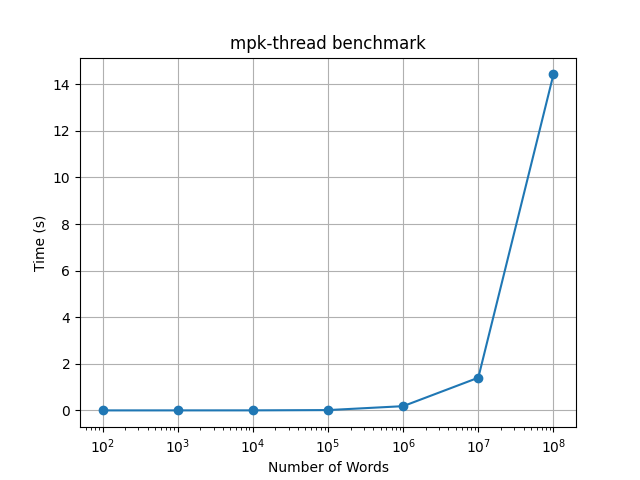
\includegraphics[width=0.3\textwidth]{../benchmark/2024-12-08_17-19-30/mpk-thread.png}
    \caption{Benchmarking MPKLink}
\end{figure}

As shown in Figure 1, MPKLink performs well for small inter-service communications but demonstrates an exponential increase in processing time when handling larger payloads, particularly between 10 million and 100 million words. This sharp rise in latency makes MPKLink, in its current form, infeasible for large bulk communications.

\begin{figure}[h]
    \centering
    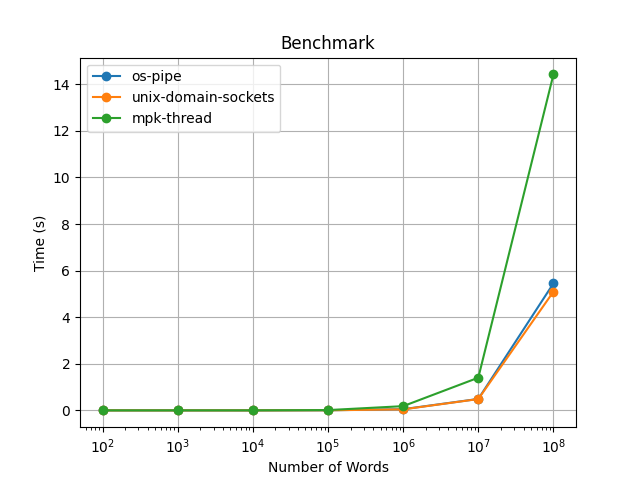
\includegraphics[width=0.3\textwidth]{../benchmark/2024-12-08_17-19-30/overview.png}
    \caption{Overview of all results for all four IPC methods}
\end{figure}

Figure 2 provides a comparative overview of MPKLink and the other three IPC communication methods. While MPKLink achieves similar performance to its counterparts, it is not faster than any of them across the range of word counts tested.

\begin{figure}[h]
    \centering
    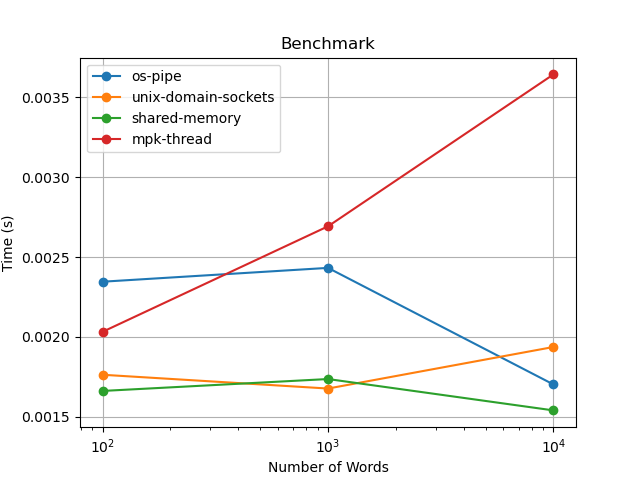
\includegraphics[width=0.3\textwidth]{../benchmark/2024-12-08_17-19-30/overview2.png}
    \caption{Overview of small results for all four IPC methods}
\end{figure}

In Figure 3, we focus on smaller inter-service communications (10000 words or fewer). Here, MPKLink outperforms OS pipes by approximately 0.0005 seconds (for small communications of 100 words or fewer) but still falls behind shared memory and UNIX domain sockets. However, MPKLink offers stronger isolation guarantees than shared memory, making it a suitable choice in scenarios where security and isolation are critical. Additionally, the architecture of MPKLink—sharing memory between two services running on individual threads via an mmap-based region—allows it to handle larger communications effectively. In contrast, the baseline shared memory approach cannot handle requests of 100,000 words or more.

\begin{table}[h!]
    \centering
    \label{tab:ipc-best}
    \begin{tabular}{|r|l|l|}
        \toprule
        \hline
        \textbf{Word Count} & \textbf{MPKLink (s)} & \textbf{Best Other (s)} \\
        \midrule
        100       & 0.00203        & 0.00166 (Shared Memory) \\
        1,000     & 0.00269        & 0.00168 (Unix Sockets) \\
        10,000    & 0.00364        & 0.00154 (Shared Memory) \\
        100,000   & 0.01536        & 0.00660 (OS Pipe) \\
        1,000,000 & 0.18374        & 0.04571 (Unix Sockets) \\
        10,000,000 & 1.40530       & 0.48885 (Unix Sockets) \\
        100,000,000 & 14.42533     & 5.10027 (Unix Sockets) \\
        \hline
        \bottomrule
    \end{tabular}
    \caption{Comparison of MPKLink and Best-Performing IPC}
\end{table}

Finally, we provide a side-by-side comparison of MPKLink with the best-performing IPC method for each word count. While MPKLink shows competitive performance for small payloads, it is consistently slower than the best-performing alternatives, especially as the word count increases.


\section{Related Work}
Previous research involving Intel Memory Protection Keys (MPK) has primarily focused on memory protection at rest, addressing the isolation and integrity of data within a single process rather than for inter-process communication.
Two notable works in this area are \textbf{ERIM}\cite{vahldiek2019erim} and \textbf{Hodor}\cite{hedayati2019hodor}, which combine MPK with binary introspection and hardware watchpoints to enforce intra-process isolation.
These systems are designed to protect sensitive data by dynamically adjusting memory access rights within a process.
While they provide significant improvements in security by isolating memory regions, their focus is on safeguarding data at rest, such as protecting static memory segments or mitigating potential attacks on individual processes.
These approaches do not extend to managing data in transit between processes, which is the focus of our work with MPKLink.

In contrast to these studies, our research explores the use of Intel MPK for communication between co-located microservices, specifically addressing data in transit.
While studies such as \textbf{Performance Characterization of Communication Protocols in Microservice Applications} and \textbf{Serverless Computing: An Investigation of Factors Influencing Microservice Performance} have extensively analyzed the performance of traditional communication protocols like REST and gRPC within microservices architectures, they do not consider the potential of MPK for enhancing communication efficiency and security.
These studies focus on optimizing communication mechanisms and identifying performance bottlenecks in microservices, but they do not explore the benefits of shared memory communication with fine-grained access control provided by MPK.
Our work builds on these findings by proposing a practical and secure framework for using MPK to protect memory regions used for inter-microservice communication, offering both performance gains and enhanced security guarantees.


%-------------------------------------------------------------------------------
\section*{Acknowledgments}
This project was conducted as part of the CS 239: Efficient Cryptography-Based Systems course at UCLA during the Fall 2024 quarter.
We would like to thank Prof.
Sam Kumar for his guidance and support throughout the project in addition to his instruction in the course.

%-------------------------------------------------------------------------------
\section*{Availability}
The source code for MPKLink and relevant benchmarks are open-sourced and available at \url{https://github.com/ssalandary/MPKLink}.

%-------------------------------------------------------------------------------
\bibliographystyle{plain}
\bibliography{sources.bib}

%%%%%%%%%%%%%%%%%%%%%%%%%%%%%%%%%%%%%%%%%%%%%%%%%%%%%%%%%%%%%%%%%%%%%%%%%%%%%%%%
\end{document}
%%%%%%%%%%%%%%%%%%%%%%%%%%%%%%%%%%%%%%%%%%%%%%%%%%%%%%%%%%%%%%%%%%%%%%%%%%%%%%%%

%%  LocalWords:  endnotes includegraphics fread ptr nobj noindent
%%  LocalWords:  pdflatex acks